\label{machineLearning}
A part of this thesis was the categorization of the scraped pages. Categorization in this context means the procedure of assigning categories (labels) to pages. The data set at hand contained a vast amount of pages, as we discussed in chapter \ref{datasetAnalysis}. The manual categorization of this number of pages would therefore take too much time and in consequence was infeasible. An automatic system for text classification was required. A simple system with a list of words assigned to each label was introduced but was performing poorly. A more sophisticated tool for text categorization is machine learning. We decided to use supervised machine learning (ML).

This chapter describes ML in general. Secondly, the main approaches of ML, reinforcement learning(RLr), unsupervised learning (ULr), and supervised learning (SLr), are characterized. Lastly we depict what an artificial neural network (ANN) is. The approach used in this thesis is an ANN using SLr.
 
\section{Machine learning} \label{machineLearning}
The term \textit{machine learning} was first introduced by Arthur Samuel. In his paper \textit{Some Studies in Machine Learning Using the Game of Checkers} \cite{machineLearningOriginal} he proved it is possible for a program to develop better game-related skills than the skills of the programmer of the program.

ML is the procedure in which an agent creates a model which develops the ability to perform a certain task at least as well as a human would. The learning process is based on the evaluation of gained experience \cite{machineLearningToday}. The agent requires an initial data set in order to train and validate. The size of initial the data set depends on the nature of the task and the selected ML type and set of algorithms. During training the agent attempts to perform the given task and validates its own performance. The agent then adjusts its criteria for performing the task based on the validation results. These two steps are repeated a number of times defined by the programmer. The output of the agent is a model able to perform the task it was trained for. 

ML is used across various industries and fields. The need for automated analysis is increasing with the growing popularity of \textit{big data}\footnote{A data set too vast or complex for traditional or manual data processing.} \cite{bigDataExplained} \cite{bigDataPopularity}. ML is used widely with Big Data. Another use for ML is in the automotive industry. Cars with assisted parking or breaking, or self-driving cars are examples\cite{selfDrivingCars}. Also, ML is used frequently in games for a more natural game experience \cite{machineLearningGaming}. 

There are several approaches in ML based on the different ways of training. We describe the three main approaches in the subsections following. Namely \textit{reinforcement learning} in subsection \ref{reinforcementLearning}, \textit{unsupervised learning} in subsection \ref{unsupervisedLearning}, and \textit{supervised learning} in subsection \ref{supervisedLearning}. The approach used in this thesis was \textit{supervised learning}. 

\subsection{Reinforcement learning} \label{reinforcementLearning}
It is suitable to use RLr if behaviours in dynamic environments are to be learned \cite{reinforcementLearningIntroduction}. A software agent receives an indication of the state of the environment. The agent then pics an action from a discrete set of agent actions. Next the state is modified by the action. The value of this modification is passed on as a scalar reinforcement signal to the agent. The objective for the agent is to maximize the long-run total of reinforcement signal values. This is achieved over time by leveraging a number of specialized algorithms together with methodical trial and error.

\subsection{Unsupervised learning} \label{unsupervisedLearning}
 ULr is used when seeking common patterns or relationships in data. It is also commonly used when trying to find anomalies in data. ULr in context of ML is inspired by the neurons in our brains and the way our brains learn without external instructions \cite{unsupervisedLearningIntroduction}. The software agent receives an unlabeled data set as input. The agent breaks the data down to critical components using specialized algorithms. It then identifies similarities and divides the data into groups. No feedback is involved.

\subsection{Supervised learning} \label{supervisedLearning}
SLr is suitable to use for the classification of data. During training SLr relies on labeled data \cite{machineLeraningApproaches}. The input of the software agent of SLr is a labeled data set. The software agent divides the data---label pairs into a a training and test set randomly. The agent is to find a function with the data as input and the correct label as output. To achieve this the agent is trained on the training set and validated using the test set. After each run the accuracy and loss is computed and the function is modified with the goal to improve the future output. 

\section{Artificial neural networks} \label{artificialNeuralNetworks}
An ANN is a ML system inspired by animal brains \cite{machineLeraningApproaches}. A brain is composed of components such as neurons. Neurons communicate with each other by passing information through synapses. The more often two neurons communicate the stronger the synapses between them are \cite{neuronsInBrain}. This results in a neuron prioritizing information passed by neurons participating in frequent communication. 

An ANN is comprised of layers of nodes sometimes also called \textit{neurons}. The neurons communicate via directed links of various relevance also called \textit{weight}. The weight is represented by a real number. A neuron determines whether to react to information gathered through a link according to its weight passed to an \textit{activation function}. We discuss activation functions later in subsection \ref{activationFunction}. Neurons exist in groups called \textit{layers}. Layers used in this thesis were \textit{convolutional layers} \ref{convolutionalLayers}, \textit{polling layers} \ref{poolingLayers}, and \textit{dense layers} \ref{denseLayers}. All of the used layers are described closer in the next subsections. 

One learning cycle is called an \textit{epoch}. In this paragraph we characterize a typical epoch in an ANN using SLr. At the beginning of an epoch the training data is passed to the first layer. Data is passed from one layer to the next one. Every layer modifies the received data before passing it on. The manner in which the data is modified depends on the type of the layer. After the data is processed by the last layer the output model is evaluated using the testing data. Improving the model is now the objective. A way leveraged to improve accuracy is the calculation of the loss by utilizing a \textit{loss function}. The loss function is outlined in more detail in subsection \ref{lossFunction}. After evaluating the loss the weights of the neurons are adjusted by the \textit{backward propagation of errors} detailed in subsection \ref{backpropagation}. After the weights of the first layer have been adjusted the epoch ends. The number of epochs is specified by the programmer. 

\subsection{Convolutional layer}\label{convolutionalLayers}
\begin{figure}[ht!]
  \centering
  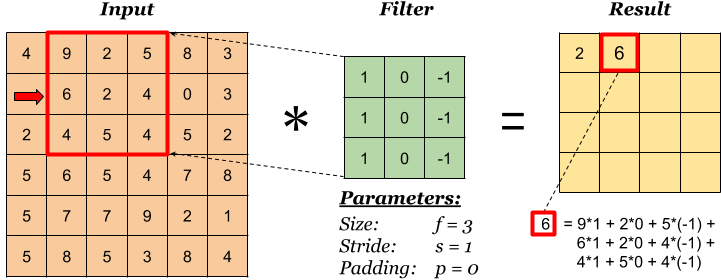
\includegraphics[width=\textwidth]{Images/convolution-operation.png}
  \caption{The visualized process of a ConvO \cite{convolutionOperationVisualization}. The very left square is the input of an 2D image of size 6x6 pixels. The square in the center depicts the 3x3 kernel with no padding. The stride of the kernel is 3 pixels. The very right square represents the partial result after the kernel was applied to two sections of the input. The final output will be of size 4x4 pixels. The ConvO itself is enumerated under the output image.} 
  \label{convolutionalLayerVisualization}
\end{figure} 
Convolutional layers (ConvL) are suited for finding features in data~\cite{CNN}. A ConvL decreases the~ size and complexity of~the~input. It does so by sliding a \textit{filter}, also called kernel, of a certain size with a certain stride across the input. The stride size represents the number of input-units, e.g. pixels, the kernel, needs to skip in order to perform the next step\footnote{The sliding direction is to the right. If sliding to the right is not possible the filter is returned to the very left and stride-size down. If sliding down is not viable the pooling is finished.}. The kernel is represented by real numbers. The kernel is applied to a portion of the image corresponding to the kernel size, called the \textit{receptive field}~\cite{receptiveField}. This action is called a \textit{convolution operation} (ConvO). After applying the kernel to all possible reception fields the output is generally smaller in size than the input. It is, however, possible for the output dimensions to be the same as the input dimensions. Moreover, the information carried in the borders of the input may not be lost. This is useful when the number of ConcLs is rather sizable. This is achieved by applying \textit{padding}. Padding is the practice of adding information around the borders of the input, e.g. \textit{zero-padding}\footnote{Zero-padding is a specific type of padding. The input is enriched with zeros around the borders.}.

An example of a simple ConvO is visualized in figure~\ref{convolutionalLayerVisualization}. 


\subsection{Pooling layer}\label{poolingLayers}
\begin{figure}[ht!]
  \centering
  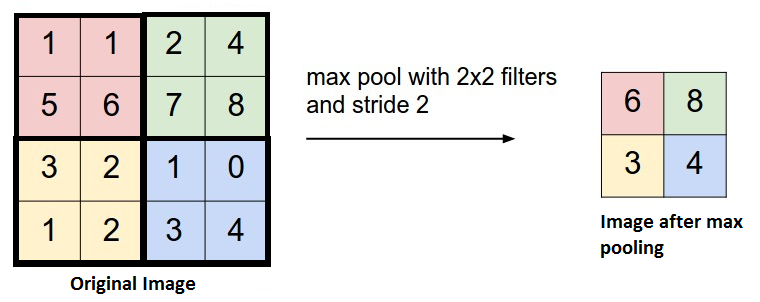
\includegraphics[width=\textwidth]{Images/maxPooling.png}
  \caption{The visualized process of max-pooling with filter size of 2x2 pixels and stride length of 2 pixels by Analytics Vidhya~\cite{maxPoolingVisualization}. The input is a 2D image and is depicted by a square with scalar values. The size of the image is 4x4 pixels. The square on the right is the result after max-pooling is applied on the input. The output image is of size 2x2 pixels. The max-pooling process is described in subsection \ref{poolingLayers}.} 
  \label{maxPoolingVisualization}
\end{figure} 
Pooling layers (PoolL) reduce the size of the input by down-sampling. The procedure resembles a sliding window of a certain size sliding over the input with a certain stride. The stride in this layer is similar to the stride in ConvLs \ref{convolutionalLayers}. The result of each step of the pooling depends on the method used. There are several types of methods to choose from for the PooL. One of the most used type is \textit{max-pooling} \cite{CNN}. The return value of max-pooling is the maximum value from the values in the currenlty present in the filter. After applying the filter to all input portions the result is passed to the next layer.

A simple example case of max-pooling is shown in figure \ref{maxPoolingVisualization}. We now describe the operation of max-pooling on the previously mentioned figure. In the beginning the upper left corner of the filter is set to be in the upper left corner of the input which is the red part of the image. The maximum value from the values \textit{1; 1; 5; 6;} is \textit{6}. The filter therefore returns the red result \textit{6}. Next the upper left corner of the filter moves two pixels to the right. It now occupies the green part of the input image. It again performs the max-pooling operation. It is not possible for the filter to slide right anymore as the end of the input was reached. The filter is therefore returned to the beginning of the line and moved two pixels down into the yellow portion. After returning the yellow result the filter slides two pixels to the right and once more return the maximum value. It is not possible to move the filter right nor down. The Max-pooling now is finished an the result is the square on the right.
\subsection{Dense layer}\label{denseLayers}
(DnsL)
\subsection{Activation function}\label{activationFunction}
(AcF)
\subsection{Loss function}\label{lossFunction}
(LsF)
\subsection{Backward propagation of error}\label{backpropagation}
Backward propagation of error  (backpropagation)
